% !TeX program = xelatex
% !TeX encoding = UTF-8
\documentclass[aspectratio=169,11pt]{beamer}

% Compile with XeLaTeX.
\usepackage{iftex}
\ifPDFTeX
  \usepackage[T1]{fontenc}
  \usepackage[utf8]{inputenc}
\else
  \usepackage{fontspec}
  \setsansfont{DejaVu Sans}
  \renewcommand{\familydefault}{\sfdefault}
\fi

\usepackage{graphicx}
\usepackage{booktabs}
\usepackage{tabularx}
\usepackage{array}
\usepackage{ragged2e}
\usepackage{tikz}
\usepackage{hyperref}
\usepackage{adjustbox}
\usepackage{microtype}

\usetikzlibrary{positioning,arrows.meta,calc}

% ---------- Visual system ----------
\definecolor{Ink}{HTML}{17212B}
\definecolor{Muted}{HTML}{667085}
\definecolor{Soft}{HTML}{F3F6FA}
\definecolor{Line}{HTML}{D9E1EA}
\definecolor{Accent}{HTML}{2454D6}
\definecolor{AccentTwo}{HTML}{0E8A7A}
\definecolor{Warning}{HTML}{B54708}

\setbeamertemplate{navigation symbols}{}
\setbeamertemplate{itemize item}{\color{Accent}\small$\blacktriangleright$}
\setbeamertemplate{itemize subitem}{\color{AccentTwo}\scriptsize$\bullet$}
\setbeamertemplate{enumerate item}{\color{Accent}\insertenumlabel.}
\setbeamercolor{normal text}{fg=Ink,bg=white}
\setbeamercolor{frametitle}{fg=Ink,bg=white}
\setbeamerfont{frametitle}{size=\Large,series=\bfseries}
\setbeamerfont{framesubtitle}{size=\normalsize,series=\mdseries}
\setbeamercolor{structure}{fg=Accent}
\setlength{\parskip}{0.25em}

\setbeamertemplate{frametitle}{%
  \vspace{0.35cm}
  \begin{beamercolorbox}[wd=\paperwidth,leftskip=0.7cm,rightskip=0.7cm]{frametitle}
    \insertframetitle
    \ifx\insertframesubtitle\empty\else\par{\usebeamerfont{framesubtitle}\color{Muted}\insertframesubtitle}\fi
  \end{beamercolorbox}
  \vspace{-0.15cm}
}

\setbeamertemplate{footline}{%
  \leavevmode%
  \hbox{%
    \begin{beamercolorbox}[wd=.68\paperwidth,ht=2.7ex,dp=1.2ex,leftskip=.7cm]{author in head/foot}%
      \color{Muted}\scriptsize LLM Labels, KMeans Clusters, and Discourse Form
    \end{beamercolorbox}%
    \begin{beamercolorbox}[wd=.32\paperwidth,ht=2.7ex,dp=1.2ex,rightskip=.7cm plus1fil]{date in head/foot}%
      \hfill\color{Muted}\scriptsize \insertframenumber/\inserttotalframenumber
    \end{beamercolorbox}}
  \vskip0pt%
}

\newcommand{\code}[1]{\texttt{#1}}
\newcommand{\key}[1]{\textcolor{Accent}{\textbf{#1}}}
\newcommand{\muted}[1]{\textcolor{Muted}{#1}}
\newcommand{\smallcap}[1]{\textcolor{Muted}{\scriptsize\MakeUppercase{#1}}}

\newcommand{\sectiontag}[1]{%
  \tikz[baseline=(x.base)]\node[fill=Soft,draw=Line,rounded corners=8pt,inner xsep=7pt,inner ysep=3pt](x){\scriptsize\color{Muted}#1};%
}

\newcommand{\statement}[1]{%
  \begin{center}
  \begin{tikzpicture}
    \node[fill=Soft, draw=Line, rounded corners=5pt, inner xsep=12pt, inner ysep=9pt, text width=.86\linewidth, align=center] {\large\bfseries #1};
  \end{tikzpicture}
  \end{center}
}

\newcommand{\safeinclude}[2][0.88\linewidth]{%
  \IfFileExists{#2}{%
    \includegraphics[width=#1]{#2}%
  }{%
    \begin{tikzpicture}
      \node[draw=Line, fill=Soft, rounded corners=5pt, minimum width=#1, minimum height=0.44\textheight, align=center, text width=.72\linewidth] {\color{Muted}\Large Figure placeholder\\[0.3em]\scriptsize\texttt{\detokenize{#2}}};
    \end{tikzpicture}%
  }%
}

\title{Auditing LLM Topic Labels with Unsupervised Text Clustering}
\subtitle{Canadian Parliamentary Speeches, 1920--1949}
\author{Your Name}
\institute{Evaluating Econometric Methods}
\date{\today}

\begin{document}

% ---------- 1 ----------
\begin{frame}[plain]
  \begin{tikzpicture}[remember picture,overlay]
    \fill[Accent] (current page.north west) rectangle ([xshift=0.18cm]current page.south west);
    \fill[Soft] ([xshift=0.18cm]current page.north west) rectangle ([xshift=1.2cm]current page.south west);
  \end{tikzpicture}
  \vspace{0.85cm}
  \hspace{0.65cm}\sectiontag{Research Presentation}

  \vspace{0.45cm}
  \hspace{0.65cm}\begin{minipage}{0.80\linewidth}
    {\fontsize{25}{29}\selectfont\bfseries\begin{tabular}{@{}l@{}}Auditing LLM Topic Labels\\with Unsupervised\\Text Clustering\end{tabular}}\par
    \vspace{0.32cm}
    {\Large\color{Muted}\raggedright Canadian Parliamentary Speeches, 1920--1949}\par
    \vspace{0.75cm}
    {\large Your Name}\par
    \vspace{0.10cm}
    {\color{Muted}Evaluating Econometric Methods \; | \; \today}
  \end{minipage}
\end{frame}

% ---------- 2 ----------
\begin{frame}{The Core Argument}
\statement{LLM labels and KMeans clusters should not be treated as competing answers to the same question.}

\vspace{0.25cm}
\begin{columns}[T,onlytextwidth]
  \begin{column}{0.47\textwidth}
    \smallcap{LLM labels}
    \vspace{0.15cm}
    \begin{itemize}
      \item classify speeches by \key{policy content};
      \item provide broad, interpretable topic categories;
      \item serve as provisional semantic reference labels.
    \end{itemize}
  \end{column}
  \begin{column}{0.47\textwidth}
    \smallcap{KMeans clusters}
    \vspace{0.15cm}
    \begin{itemize}
      \item group speeches by \key{lexical similarity};
      \item reveal repeated forms of parliamentary language;
      \item expose discourse structures inside and across topics.
    \end{itemize}
  \end{column}
\end{columns}
\end{frame}

% ---------- 3 ----------
\begin{frame}{Reframing the Question}
\begin{columns}[T,onlytextwidth]
  \begin{column}{0.48\textwidth}
    \smallcap{Initial question}
    \vspace{0.15cm}
    \statement{Is KMeans less accurate than LLM topic labeling?}
    \vspace{-0.1cm}
    \muted{This framing is too narrow, because it assumes that both methods are trying to recover the same object.}
  \end{column}
  \begin{column}{0.48\textwidth}
    \smallcap{Revised question}
    \vspace{0.15cm}
    \statement{What does KMeans reveal that LLM topic labels do not show?}
    \vspace{-0.1cm}
    \muted{This framing turns mismatches into evidence about the structure of political language.}
  \end{column}
\end{columns}
\end{frame}

% ---------- 4 ----------
\begin{frame}{Final Research Question}
\vspace{0.2cm}
\statement{When LLM-generated labels classify parliamentary speeches by policy content, what additional information can KMeans clusters provide about the discourse form of those speeches?}

\vspace{0.3cm}
\begin{itemize}
  \item The LLM label answers: \key{what policy topic is being discussed?}
  \item The KMeans cluster answers: \key{what kind of language is used to discuss it?}
  \item The main empirical object is therefore not simple agreement or disagreement, but the pattern of \key{structured mismatch}.
\end{itemize}
\end{frame}

% ---------- 5 ----------
\begin{frame}{Data and Key Variables}
\small
\begin{tabularx}{\textwidth}{>{\raggedright\arraybackslash}p{0.27\textwidth}X}
\toprule
\textbf{Variable} & \textbf{Role in the analysis} \\
\midrule
\code{speechtext} & cleaned speech text used for modeling \\
\code{speechtext\_original} & original text used for close reading and interpretation \\
\code{year} & year of speech, used for period and trend analysis \\
\code{topic} & original parliamentary topic description \\
\code{category} & LLM-generated broad policy topic label \\
\code{kmeans\_cluster} & unsupervised cluster assignment from TF-IDF + KMeans \\
\code{cluster\_type} & researcher-interpreted discourse type based on cluster meaning \\
\bottomrule
\end{tabularx}

\vspace{0.35cm}
\muted{Final full-corpus output: approximately 161,633 matched speeches from Canadian parliamentary debates, 1920--1949.}
\end{frame}

% ---------- 6 ----------
\begin{frame}{Research Workflow}
\centering
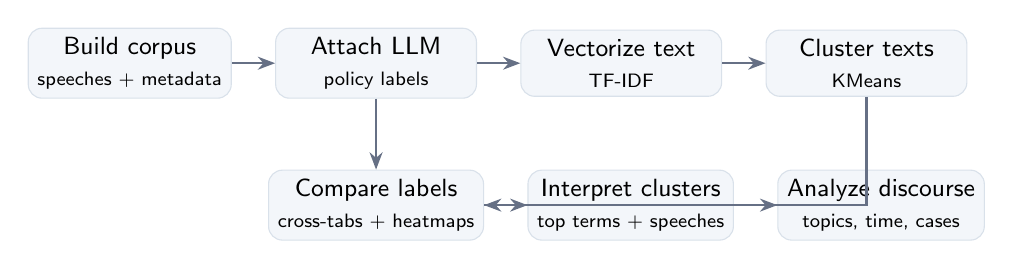
\begin{tikzpicture}[node distance=0.55cm, every node/.style={font=\small}]
  \tikzstyle{box}=[draw=Line, fill=Soft, rounded corners=5pt, minimum width=2.55cm, minimum height=0.8cm, align=center]
  \tikzstyle{arrow}=[-{Stealth[length=2.2mm]}, thick, color=Muted]

  \node[box] (a) {Build corpus\\\scriptsize speeches + metadata};
  \node[box, right=of a] (b) {Attach LLM\\\scriptsize policy labels};
  \node[box, right=of b] (c) {Vectorize text\\\scriptsize TF-IDF};
  \node[box, right=of c] (d) {Cluster texts\\\scriptsize KMeans};
  \node[box, below=0.9cm of b] (e) {Compare labels\\\scriptsize cross-tabs + heatmaps};
  \node[box, right=of e] (f) {Interpret clusters\\\scriptsize top terms + speeches};
  \node[box, right=of f] (g) {Analyze discourse\\\scriptsize topics, time, cases};

  \draw[arrow] (a) -- (b);
  \draw[arrow] (b) -- (c);
  \draw[arrow] (c) -- (d);
  \draw[arrow] (d) |- (e);
  \draw[arrow] (b) -- (e);
  \draw[arrow] (e) -- (f);
  \draw[arrow] (f) -- (g);
\end{tikzpicture}

\vspace{0.4cm}
\muted{The workflow treats LLM labels as useful but auditable, not as unquestioned ground truth.}
\end{frame}

% ---------- 7 ----------
\begin{frame}{Text Representation and Clustering}
\begin{columns}[T,onlytextwidth]
  \begin{column}{0.47\textwidth}
    \smallcap{Modeling choice}
    \begin{itemize}
      \item Cleaned speeches are represented with TF-IDF features.
      \item KMeans is estimated with 20 clusters.
      \item The clustering is unsupervised: it does not use the LLM labels as training targets.
    \end{itemize}
  \end{column}
  \begin{column}{0.48\textwidth}
    \smallcap{Interpretation strategy}
    \begin{itemize}
      \item inspect top TF-IDF terms;
      \item compare cluster-category distributions;
      \item read representative original speeches;
      \item assign historically meaningful discourse interpretations.
    \end{itemize}
  \end{column}
\end{columns}

\vspace{0.25cm}
\statement{The model is not designed to replace topic labels; it is designed to expose recurring patterns of language use.}
\vspace{-0.05cm}
\muted{KMeans settings: 20 clusters, k-means++ initialization, 300 maximum iterations, 10 initializations, random seed 42.}
\end{frame}

% ---------- 8 ----------
\begin{frame}{How the Two Labeling Systems Are Compared}
\begin{columns}[T,onlytextwidth]
  \begin{column}{0.48\textwidth}
    \smallcap{Category to cluster}
    \vspace{0.15cm}
    \begin{itemize}
      \item Start from an LLM policy category.
      \item Ask whether its speeches concentrate in one cluster or spread across several clusters.
      \item This tests whether a broad topic is linguistically homogeneous.
    \end{itemize}
  \end{column}
  \begin{column}{0.48\textwidth}
    \smallcap{Cluster to category}
    \vspace{0.15cm}
    \begin{itemize}
      \item Start from a KMeans cluster.
      \item Ask whether it corresponds to one policy field or cuts across several fields.
      \item This identifies topic-specific clusters and cross-topic discourse forms.
    \end{itemize}
  \end{column}
\end{columns}

\vspace{0.25cm}
\statement{The most informative cases are not only high-alignment clusters, but also systematic mismatches.}
\end{frame}

% ---------- 9 ----------
\begin{frame}{Finding 1: Some Clusters Align Clearly with Policy Topics}
\small
\begin{tabularx}{\textwidth}{>{\raggedleft\arraybackslash}p{0.13\textwidth}X X}
\toprule
\textbf{Cluster} & \textbf{Characteristic vocabulary} & \textbf{Dominant LLM category} \\
\midrule
19 & tariff, duty, import, protection & International Trade and Tariffs \\
9 & railway, line, Canadian National & Transportation and Communications \\
4 & tax, income, revenue, taxation & Public Finance and Taxation \\
17 & wheat, grain, bushel, wheat board & Agriculture and Food Policy \\
2 & bank, loan, credit, money & Banking and Monetary Policy \\
\bottomrule
\end{tabularx}

\vspace{0.35cm}
\statement{Alignment is strongest when a policy field has distinctive, repeated, technical vocabulary.}
\end{frame}

% ---------- 10 ----------
\begin{frame}{Finding 2: A Single LLM Category Can Contain Multiple Discourse Forms}
\begin{columns}[T,onlytextwidth]
  \begin{column}{0.47\textwidth}
    \smallcap{Example: Agriculture and Food Policy}
    \begin{itemize}
      \item wheat and grain policy;
      \item farm prices and agricultural markets;
      \item inspection and product regulation;
      \item export rules;
      \item legal authority;
      \item federal-provincial administration;
      \item general parliamentary debate.
    \end{itemize}
  \end{column}
  \begin{column}{0.48\textwidth}
    \smallcap{Interpretation}
    \vspace{0.15cm}
    \statement{The LLM category is semantically reasonable, but it hides the internal language structure of the topic.}
    \vspace{-0.15cm}
    \muted{KMeans separates different ways of speaking within the same policy area.}
  \end{column}
\end{columns}
\end{frame}

% ---------- 11 ----------
\begin{frame}{Finding 3: Some Clusters Capture Cross-Topic Discourse}
\scriptsize
\begin{tabularx}{\textwidth}{>{\raggedleft\arraybackslash}p{0.15\textwidth}X X}
\toprule
\textbf{Cluster} & \textbf{Interpretation} & \textbf{Why it crosses topics} \\
\midrule
15 & general parliamentary discourse & common debate language across policy fields \\
5 & legal and legislative language & statutes, authority, clauses, regulations \\
7 & budgetary and expenditure language & appropriations, estimates, administrative costs \\
8 & committee and procedural language & motions, amendments, committee-stage discussion \\
18 & intergovernmental language & federal-provincial coordination and jurisdiction \\
\bottomrule
\end{tabularx}

\vspace{0.2cm}
\statement{A low match rate is not automatically a model failure; it may reveal a reusable parliamentary discourse form.}
\end{frame}

% ---------- 12 ----------
\begin{frame}{Close Reading: Same Topic, Different Forms}
\small
\begin{tabularx}{\textwidth}{>{\raggedright\arraybackslash}p{0.16\textwidth}X X}
\toprule
\textbf{Speech ID} & \textbf{Shared policy topic} & \textbf{KMeans interpretation} \\
\midrule
570680 & Inspection and Sale Act regulatory powers & legal and administrative authority \\
749345 & amendment of dairy produce export regulations & clause-level amendment procedure \\
\bottomrule
\end{tabularx}

\vspace{0.2cm}
\begin{columns}[T,onlytextwidth]
  \begin{column}{0.48\textwidth}
    \smallcap{Speech 570680}
    \begin{itemize}
      \item Parliament
      \item authority
      \item jurisdiction
      \item minister and officials
      \item regulations
    \end{itemize}
  \end{column}
  \begin{column}{0.48\textwidth}
    \smallcap{Speech 749345}
    \begin{itemize}
      \item simpler amendment
      \item strike out words
      \item paragraph (g)
      \item read this again
      \item procedural revision
    \end{itemize}
  \end{column}
\end{columns}

\vspace{0.1cm}
\statement{Same policy topic; different linguistic organization.}
\end{frame}

% ---------- 13 ----------
\begin{frame}{From 20 Clusters to Three Discourse Types}
\small
\begin{tabularx}{\textwidth}{>{\raggedright\arraybackslash}p{0.33\textwidth}p{0.22\textwidth}X}
\toprule
\textbf{Discourse type} & \textbf{Clusters} & \textbf{Meaning} \\
\midrule
Substantive policy discourse & 0, 1, 2, 4, 6, 9, 10, 11, 13, 14, 16, 17, 19 & concrete policy content and sector-specific vocabulary \\
Institutional-procedural discourse & 5, 7, 8, 18 & legal, budgetary, committee, administrative, and intergovernmental language \\
General parliamentary discourse & 3, 12, 15 & broad debate, party politics, government-opposition rhetoric \\
\bottomrule
\end{tabularx}

\vspace{0.35cm}
\muted{This grouping is interpretive. It is designed to make the cluster results historically readable, not to claim that the three types are automatically discovered ground truth.}
\end{frame}

% ---------- 14 ----------
\begin{frame}{Corpus-Level Pattern}
\centering
\safeinclude[0.82\linewidth]{../output/1920-1949-full-corpus-v1/figures/overall_cluster_type_share_by_year.png}

\vspace{0.25cm}
\muted{The descriptive trend suggests that substantive policy discourse becomes especially prominent during wartime, while general parliamentary language remains an important part of the corpus.}
\end{frame}

% ---------- 15 ----------
\begin{frame}{Case Study: Agriculture and Food Policy}
\centering
\safeinclude[0.78\linewidth]{../output/1920-1949-full-corpus-v1/figures/agriculture_cluster_type_share_by_year.png}

\vspace{0.15cm}
\scriptsize
\begin{tabularx}{\textwidth}{X r r r r}
\toprule
\textbf{Period} & \textbf{N} & \textbf{Substantive} & \textbf{General} & \textbf{Institutional} \\
\midrule
Postwar 1920s & 4,935 & 39.39\% & 40.65\% & 19.96\% \\
Depression 1930s & 5,546 & 41.80\% & 31.25\% & 26.96\% \\
Wartime & 5,575 & 60.41\% & 25.17\% & 14.42\% \\
Postwar reconstruction & 3,211 & 59.58\% & 25.47\% & 14.95\% \\
\bottomrule
\end{tabularx}
\end{frame}

% ---------- 16 ----------
\begin{frame}{Methodological Contribution}
\begin{columns}[T,onlytextwidth]
  \begin{column}{0.47\textwidth}
    \smallcap{What the workflow contributes}
    \begin{itemize}
      \item It audits LLM-generated labels rather than accepting them as ground truth.
      \item It distinguishes topic content from discourse form.
      \item It turns label-cluster mismatch into an interpretable object of analysis.
    \end{itemize}
  \end{column}
  \begin{column}{0.48\textwidth}
    \smallcap{What should remain cautious}
    \begin{itemize}
      \item LLM labels are provisional semantic references.
      \item KMeans captures lexical similarity, not deep semantic meaning.
      \item The three discourse types are researcher-defined interpretations.
      \item The time trends are descriptive, not causal estimates.
    \end{itemize}
  \end{column}
\end{columns}
\end{frame}

% ---------- 17 ----------
\begin{frame}{Final Takeaway}
\vspace{0.35cm}
\statement{The LLM tells us what Parliament was talking about.}
\vspace{0.15cm}
\statement{KMeans helps us see how Parliament talked about it.}

\vspace{0.45cm}
\begin{center}
{\Large\bfseries The value of KMeans is not that it replaces LLM labels,\\[0.15cm] but that it makes their blind spots analytically visible.}
\end{center}
\end{frame}

% ---------- 18 ----------
\begin{frame}[plain]
  \begin{tikzpicture}[remember picture,overlay]
    \fill[Accent] (current page.north west) rectangle ([xshift=0.18cm]current page.south west);
    \fill[Soft] ([xshift=0.18cm]current page.north west) rectangle ([xshift=1.2cm]current page.south west);
  \end{tikzpicture}
  \vspace{2.3cm}
  \hspace{0.75cm}\begin{minipage}{0.78\linewidth}
    {\Huge\bfseries Thank you}\par
    \vspace{0.45cm}
    {\Large\color{Muted}Questions and comments are welcome.}
  \end{minipage}
\end{frame}

\end{document}
